% Part IV — Examples
\section{Examples}

% Slide 10 — Example 1: Normal Variance
\begin{frame}{Normal Variance: MLE vs MoM}
  \textbf{Data:} $X_1, \ldots, X_n \sim N(\mu, \sigma^2)$

  \vspace{0.5em}
  \begin{itemize}
    \item \textbf{MLE:} $\hat{\sigma}^2_{\text{MLE}} = \frac{1}{n} \sum_{i=1}^n (X_i - \bar{X})^2$
    \item \textbf{MoM:} $\hat{\sigma}^2_{\text{MoM}} = m_2 - (\bar{X})^2$ where $m_2 = \frac{1}{n}\sum X_i^2$
    \item \textbf{Result:} Both give the same estimate!
  \end{itemize}

  \vspace{1em}
  \begin{center}
  \begin{adjustbox}{max height=0.40\textheight}
    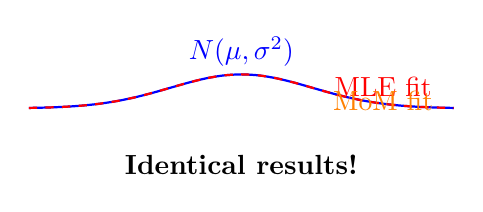
\begin{tikzpicture}[scale=0.9]
      % Normal curve
      \draw[blue, thick, domain=-3:3, smooth] plot (\x, {1.2/sqrt(2*3.14159)*exp(-0.5*\x*\x)});
      \node[blue] at (0, 0.8) {$N(\mu, \sigma^2)$};

      % Fitted curves overlay
      \draw[red, thick, domain=-3:3, smooth, dashed] plot (\x, {1.2/sqrt(2*3.14159)*exp(-0.5*\x*\x)});

      \node[red] at (2, 0.3) {MLE fit};
      \node[orange] at (2, 0.1) {MoM fit};
      \node at (0, -0.8) {\textbf{Identical results!}};
    \end{tikzpicture}
    \end{adjustbox}
  \end{center}
\end{frame}

% Slide 11 — Example 2: Poisson
\begin{frame}{Poisson Parameter $\lambda$}
  \textbf{Data:} $X_1, \ldots, X_n \sim \text{Poisson}(\lambda)$

  \vspace{0.5em}
  \begin{itemize}
    \item \textbf{MLE:} $\hat{\lambda}_{\text{MLE}} = \bar{X}$
    \item \textbf{MoM:} $\E[X] = \lambda$, so $\hat{\lambda}_{\text{MoM}} = \bar{X}$
    \item \textbf{Result:} Another coincidence between methods
  \end{itemize}

  \vspace{1em}
  \begin{center}
  \begin{adjustbox}{max height=0.40\textheight}
    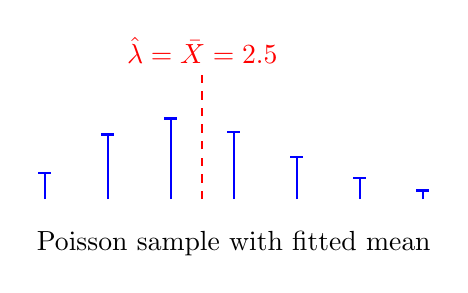
\begin{tikzpicture}[scale=0.8]
      % Histogram bars
      \foreach \x in {0,1,2,3,4,5,6} {
        \draw[blue, thick] (\x, 0) -- (\x, {exp(-2.5)*2.5^\x/factorial(\x)*5});
        \draw[blue, thick] (\x-0.1, {exp(-2.5)*2.5^\x/factorial(\x)*5}) -- (\x+0.1, {exp(-2.5)*2.5^\x/factorial(\x)*5});
      }

      % Fitted mean line
      \draw[red, thick, dashed] (2.5, 0) -- (2.5, 2);
      \node[red, above] at (2.5, 2) {$\hat{\lambda} = \bar{X} = 2.5$};

      \node at (3, -0.7) {Poisson sample with fitted mean};
    \end{tikzpicture}
    \end{adjustbox}
  \end{center}
\end{frame}

% Slide 12 — Example 3: Exponential Distribution
\begin{frame}{Exponential Parameter $\lambda$}
  \textbf{Data:} $X_1, \ldots, X_n \sim \text{Exp}(\lambda)$

  \vspace{0.5em}
  \begin{itemize}
    \item \textbf{MLE:} $\hat{\lambda}_{\text{MLE}} = \frac{1}{\bar{X}}$
    \item \textbf{MoM:} $\E[X] = \frac{1}{\lambda}$, so $\hat{\lambda}_{\text{MoM}} = \frac{1}{\bar{X}}$
    \item \textbf{Result:} Again identical! (But MLE more efficient in general)
  \end{itemize}

  \vspace{1em}
  \begin{center}
  \begin{adjustbox}{max height=0.40\textheight}
    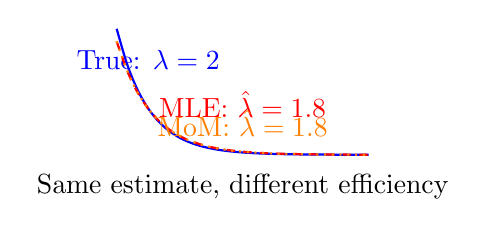
\begin{tikzpicture}[scale=0.8]
      % Exponential curves
      \draw[blue, thick, domain=0:4, smooth] plot (\x, {2*exp(-2*\x)});
      \node[blue] at (0.5, 1.5) {True: $\lambda=2$};

      \draw[red, thick, domain=0:4, smooth, dashed] plot (\x, {1.8*exp(-1.8*\x)});
      \node[red] at (2, 0.8) {MLE: $\hat{\lambda}=1.8$};

      \draw[orange, thick, domain=0:4, smooth, dotted] plot (\x, {1.8*exp(-1.8*\x)});
      \node[orange] at (2, 0.5) {MoM: $\hat{\lambda}=1.8$};

      \node at (2, -0.5) {Same estimate, different efficiency};
    \end{tikzpicture}
    \end{adjustbox}
  \end{center}
\end{frame}